% \documentclass[dvipdfmx, 11pt]{beamer}
\documentclass[aspectratio=169, dvipdfmx, 11pt]{beamer} % aspectratio=43, 149, 169
\usepackage{here, amsmath, latexsym, amssymb, bm, ascmac, mathtools, multicol, tcolorbox, subfig, bookmark}

% デザイン
\usetheme{Luebeck}
\usecolortheme{orchid}
\usefonttheme{professionalfonts}
\useinnertheme{circles}
\useoutertheme{infolines}
\setbeamercolor{title}{fg=structure, bg=}
\setbeamercolor{frametitle}{fg=structure, bg=}
\setbeamertemplate{itemize item}{\small\raise0.5pt\hbox{$\bullet$}}
\setbeamertemplate{itemize subitem}{\tiny\raise1.5pt\hbox{$\blacktriangleright$}}
\setbeamertemplate{itemize subsubitem}{\tiny\raise1.5pt\hbox{$\bigstar$}}

%しおりの文字化け解消
\usepackage{atbegshi}
\ifnum 42146=\euc"A4A2
\AtBeginShipoutFirst{\special{pdf:tounicode EUC-UCS2}}
\else
\AtBeginShipoutFirst{\special{pdf:tounicode 90ms-RKSJ-UCS2}}
\fi

\setbeamertemplate{navigation symbols}{}
\renewcommand{\kanjifamilydefault}{\gtdefault}
\newcommand{\red}[1]{\textcolor{red}{#1}}
\newcommand{\green}[1]{\textcolor{green!40!black}{#1}}
\newcommand{\blue}[1]{\textcolor{blue!80!black}{#1}}

\title[Day05]{機械学習の基礎}
\subtitle{Day05}
\author[Yudai Fujimoto]{Yudai Fujimoto}
\institute[SUS]{Suwa University of Science}
\date{\today}

\begin{document}
\maketitle

\begin{frame}{目次}
    \tableofcontents
\end{frame}

\section{主成分分析}
\begin{frame}{主成分分析}
    特徴量選択と同様に特徴量抽出を使用して、特徴量の個数を減らすことができる。\\
    特徴量選択を利用した場合は特徴量が変換されることなく、そのまま利用されていたが、
    特徴量抽出ではデータが新しい特徴量空間に射影される。
    これによって情報を保ったまま次元を下げることができ、計算量を下げることができる。
\end{frame}

\begin{frame}{主成分分析}
    ここでは主成分分析(Principal Componennt Analysis: PAC)に付いて説明する。 \\
    PCAは広く使われている教師なし、線形変換法であり、相関関係に基づいてデータをパータンから抽出するのに役立つ。
    図に示すように新しい特徴量が互いに直行するという制約の場合は、新しい部分空間の
    直交軸(主成分)を分散が最大となる方向とみなすことができる。
    \vspace{1em}
    \begin{figure}[b]
        \begin{center}
        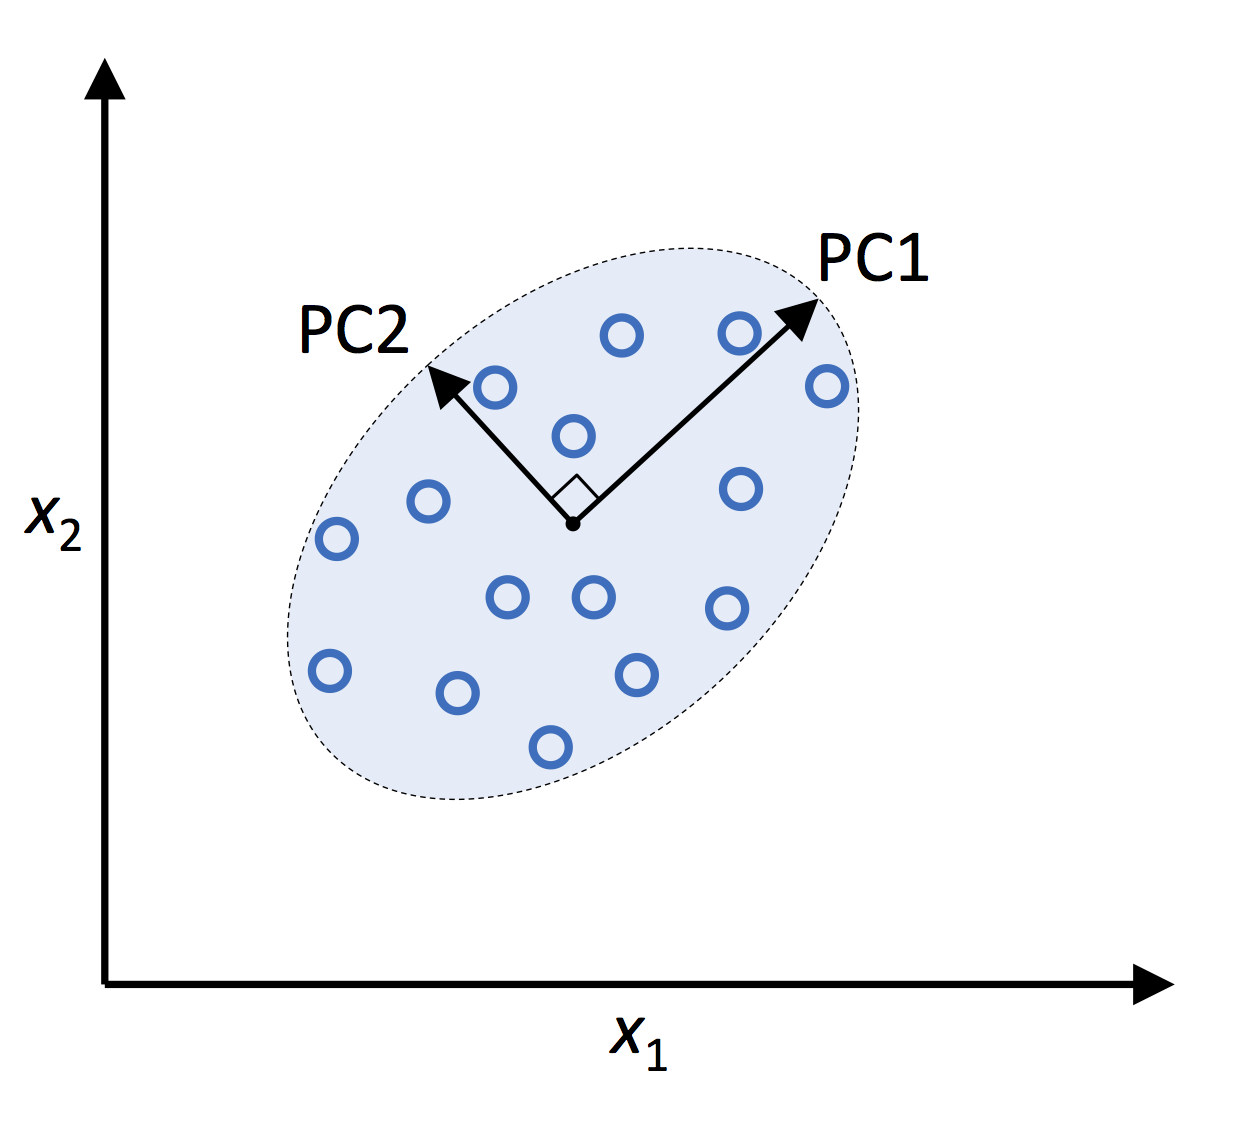
\includegraphics[width=50mm]{img/day05/fig01.png}
        \end{center}
    \end{figure}
\end{frame}

\begin{frame}{次元削減の気持ち}
    PCAを用いて次元削減を行う場合は\(d \times k\)次元の変換行列\(\bm{W}\)を作成する。 \\
    これによりベクトル\(\bm{x}\)を\(k\)次元の特徴量空間に写像できる。\\
    例として、特徴量ベクトルが次のように定義されているとする。
    \begin{equation*}
        \bm{x} = [ x_1, x_2, \ldots, x_d ], \bm{x} \in \mathbb{R}^d
    \end{equation*}
    変換行列\(\bm{x} \in \mathbb{R}^{d \times k}\)によって変換され、
    \begin{equation*}
        \bm{xW} = \bm{z}
    \end{equation*}
    次の出力ベクトルがえられる。
    \begin{equation*}
        \bm{z} = [ z_1, z_2, \ldots, z_k ], \bm{x} \in \mathbb{R}^k
    \end{equation*}
    要は、いい感じの変換行列\(\bm{W}\)を作成する
\end{frame}

\begin{frame}{主成分分析}
    PCAの流れを以下にまとめる。
    \vspace{1em}
    \begin{enumerate}
        \item \(d\)次元のデータセットを標準化する。
        \item 標準化したデータセットの共分散行列を作成する。
        \item 共分散行列を固有値ベクトルと固有値に分解する。
        \item 固有値を降順でソートすることで、対応する固有ベクトルをランク付けする。
        \item 最も大きい\(k\)個の固有値に対応する、\(k\)個のベクトルを選択する。
        \item 上位\(k\)このベクトルから射影行列を作成する。
        \item 射影行列によってデータセットを変換し、\(k\)次元のデータセットに変換する。
    \end{enumerate}
\end{frame}

\begin{frame}{スケーリング}
    PCAの方向はデータのスケールに対して敏感なので事前にデータを決まった尺度に揃えるために標準する必要がある。
    標準化は次の式を用いて、平均0、分散1、範囲が[-1, 1]になるようにする。
    \vspace{2em}
    \begin{equation*}
        x_{j}^{'} = \frac{x_j - \bar{x} _j}{\sigma_j}
    \end{equation*}
\end{frame}

\begin{frame}{共分散行列}
    次に共分散行列の作成に進む。\(d \times d\)次元の共分散行列は特徴量のペアごとの共分散を保持する。
    例えば、2つの特徴量\(x_j\)と\(x_k\)の間の共分散は、次の式を使って計算できる。
    \begin{equation*}
        \sigma_{jk} = \frac{1}{n} \sum_{i=1}^{n} (x_{j}^{(i)} - \mu_j) (x_{k}^{(i)} - \mu_k)
    \end{equation*}
    2つの特徴量の間の共分散が正になった場合は、これらの特徴量がともに増加/減少することになる。
    負の場合は逆の方向に変化することになる。\\
    共分散行列は次のように定義される。
    \begin{equation*}
        \bm{\sigma} = 
        \begin{bmatrix}
            \sigma_{1}^{2} & \sigma_{12} & \sigma_{13} \\
            \sigma_{21} & \sigma_{2}^{2} & \sigma_{23} \\
            \sigma_{31} & \sigma_{32} & \sigma_{3}^{2} \\
        \end{bmatrix}
    \end{equation*}
\end{frame}

\begin{frame}{共分散行列}
    分散行列の固有ベクトルが主成分(分散が最大となる方向)を示すのに対して、
    対応する固有値はそれらの大きさを表している。
    固有ベクトルは次の条件を満たす。
    \begin{equation*}
        \bm{\sigma} \bm{v} = \lambda \bm{v}
    \end{equation*}
    \(\lambda\)は固有値(スカラ)である。
    固有値と固有ベクトルの計算は省略する。\\
    ここで、固有値は共分散行列の特徴的な分散を示し、
    対応する固有ベクトルの重要性を示す指標となる。
\end{frame}

\begin{frame}{特徴量変換}
    共分散を固有値と固有ベクトルにうまく分解できたところで、特徴量の変換に進む。
    もっと大きい\(k\)個の固有値に対応する\(k\)個の固有ベクトルを選択し変換行列\(\bm{W}\)
    を作成する。
    \begin{equation*}
        \bm{xW} = \bm{z}
    \end{equation*}
    \begin{equation*}
        \bm{x} \in \mathbb{R}^{d}
    \end{equation*}
    \begin{equation*}
        \bm{W} \in \mathbb{R}^{d \times k}
    \end{equation*}
    \begin{equation*}
        \bm{z} \in \mathbb{R}^{k}
    \end{equation*}
    これによって特徴量を任意の次元に射影することができる。
\end{frame}

\section{線形判別分析}
\begin{frame}{線形判別分析}
    線形判別分析( Linear Discriminant Analysis: LDA)もPCA同様に正則化されていないモデルに対して、
    次元を削減し、計算効率を向上させることができる。
    PCAがデータセットに置いて分散が最も大きい直行成分を見つけ出すのに対し、
    LDAはクラス分類を最適化する特徴量空間を密陀僧とする。
    \begin{figure}[h]
        \begin{minipage}[b]{0.45\linewidth}
            \centering
            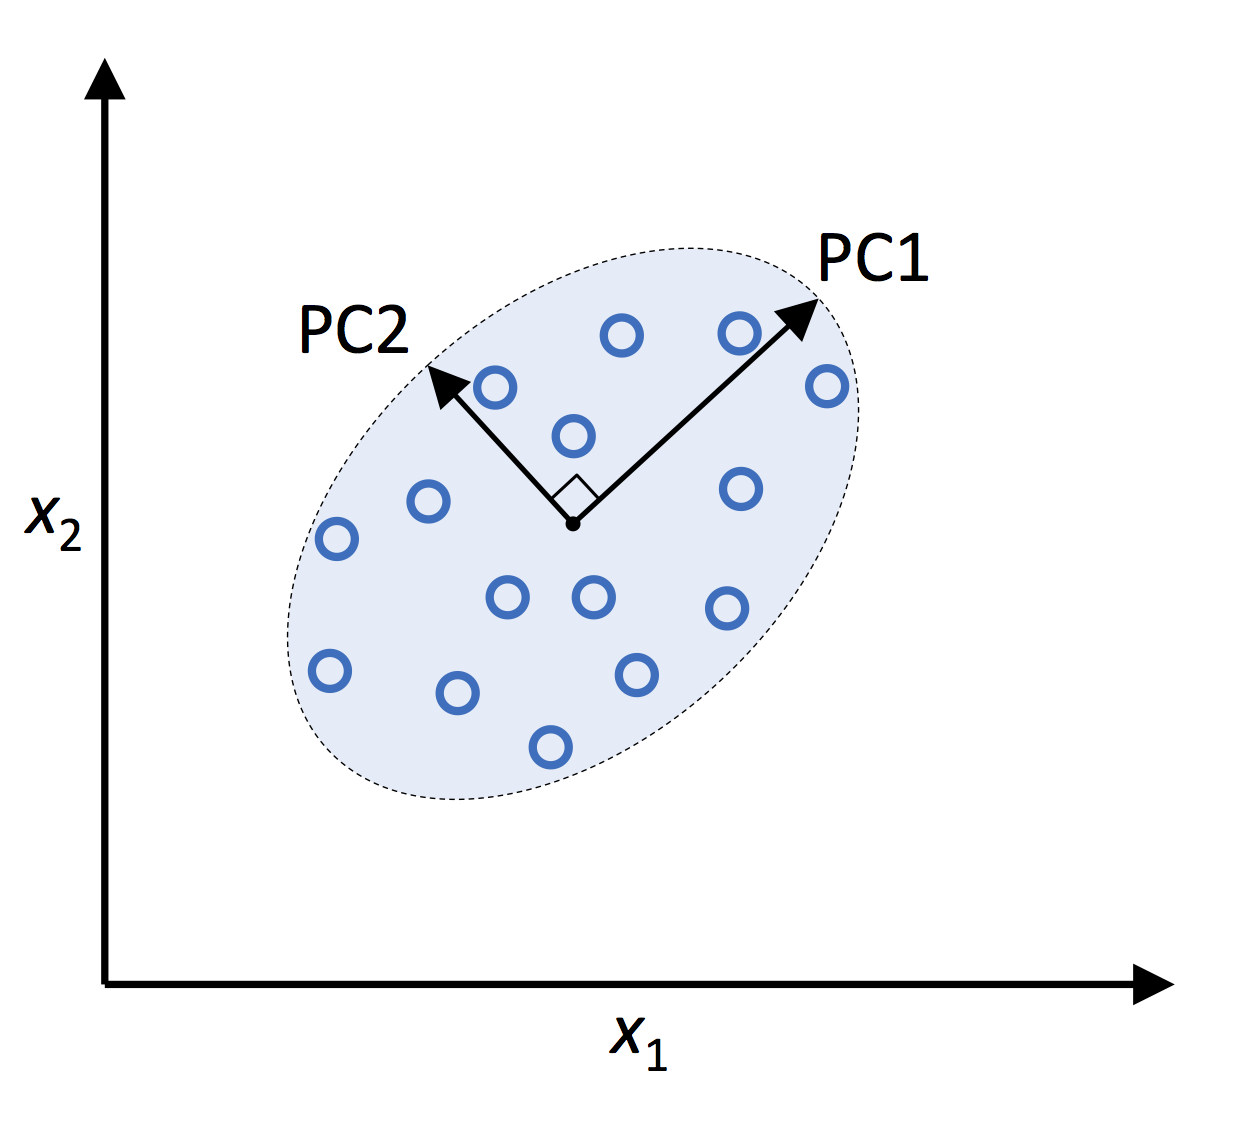
\includegraphics[width=40mm]{img/day05/fig01.png}
            \caption*{PCA}
        \end{minipage}
        \begin{minipage}[b]{0.45\linewidth}
            \centering
            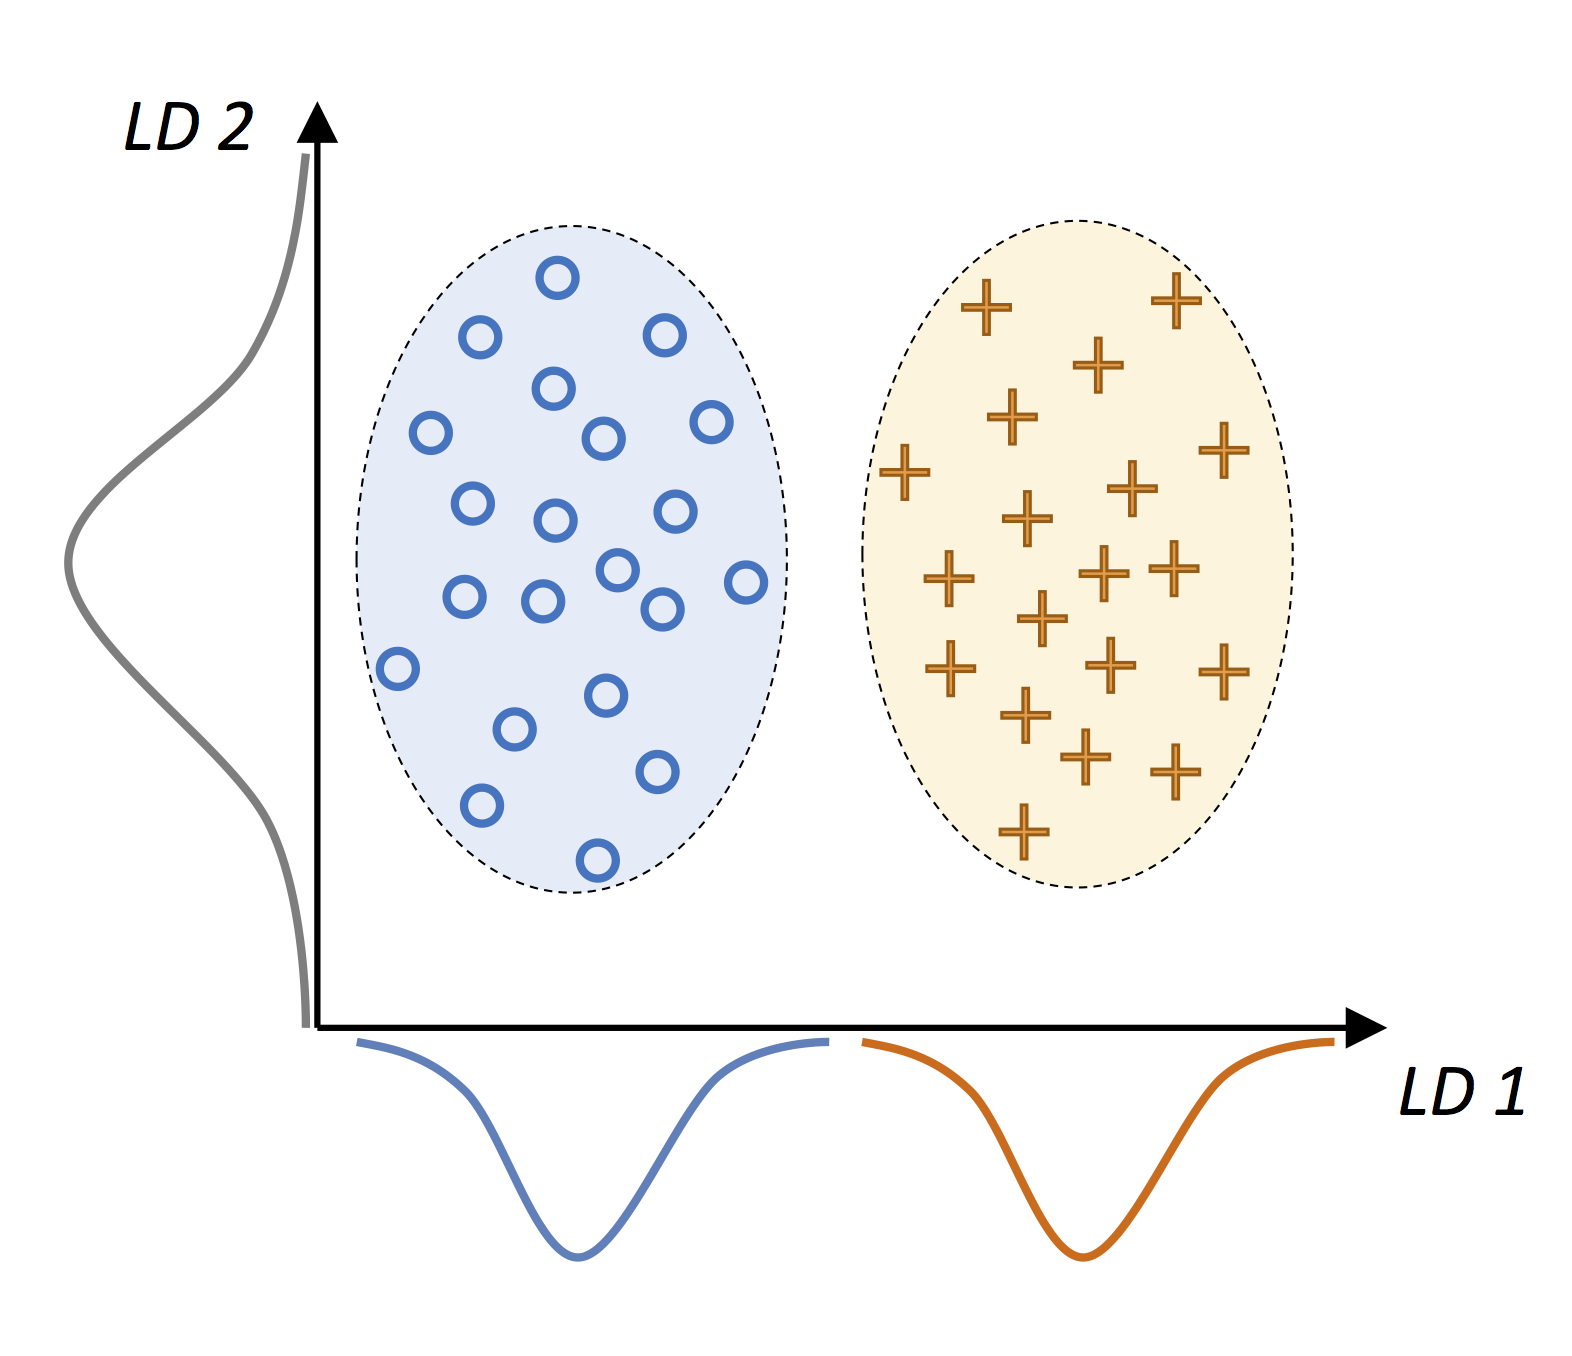
\includegraphics[width=40mm]{img/day05/fig02.png}
            \caption*{LDA}
        \end{minipage}
    \end{figure}
\end{frame}

\begin{frame}{線形判別分析}
    \(x\)軸(LD1)に示されているLDAによって正規分布に従う2つのクラスが分割されている例である。
    しかし、\(y\)軸(LD2)に示されている線形判別はクラス情報を捉えていないので良い例とは言えない。
    \begin{figure}[h]
        \centering
        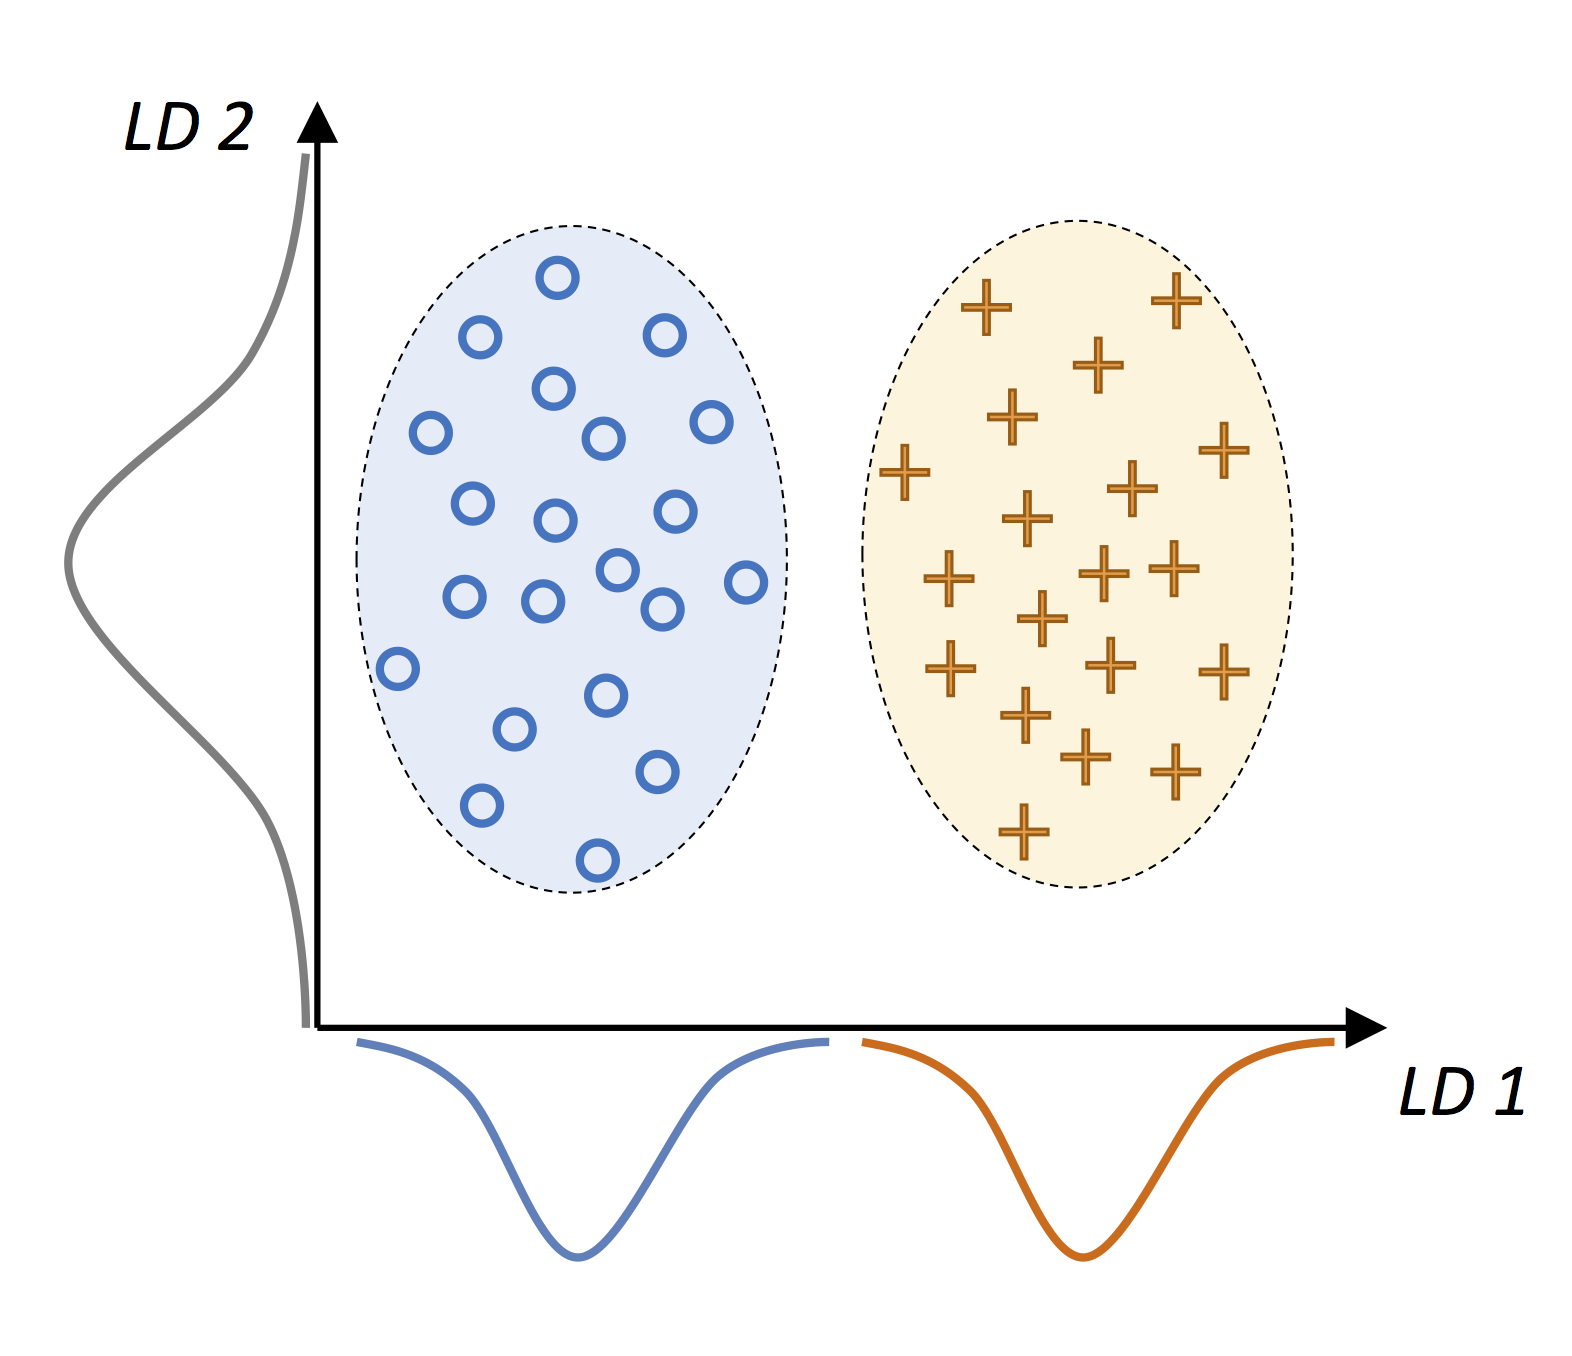
\includegraphics[width=60mm]{img/day05/fig02.png}
    \end{figure}
\end{frame}

\begin{frame}{線形判別分析}
    LDAでは以下の条件が前提となる。
    \begin{itemize}
        \item データが正規分布に従っている。
        \item クラスの共分散行列が全く同じである。
        \item 訓練データが統計学的に独立である。
    \end{itemize}
    \vspace{1em}
    しかし、多少この条件を満たしていなくても、次元削減はそれなりにうまくいく。
\end{frame}

\begin{frame}{線形判別分析}
    LDAを実行するために必要な手順をまとめておく。
    \vspace{1em}
    \begin{enumerate}
        \item \(d\)次元のデータを標準化する。(\(d\)はもとの特徴帳の次元)
        \item クラスごとに\(d\)次元の平均ベクトル(各次元の平均で)を計算する。
        \item 平均ベクトルからクラス間変動平均\(\bm(S)_B\)とクラス内変動行列\(\bm(S)_W\)を計算する。
        \item 行列\(\bm(S)_{B}^{-1} \bm(S)_W\)の固有ベクトルと対応する固有値を計算する。
        \item 固有値を降順でソートして固有ベクトルをランク付けする。
        \item 上位\(k\)このベクトルから射影行列\(\bm{W}\)を作成する。
        \item 射影行列\(\bm{W}\)を使ってデータを新しい特徴量空間へ射影する。
    \end{enumerate}
    \vspace{1em}
    このように行列を固有値と固有ベクトルに分解し、新しい特徴量空間へ射影するとことは
    PCAとよく似ている。しかし、LDAはクラスラベルを情報として利用する。
\end{frame}

\begin{frame}{線形判別分析}
    PCAに関する説明で標準化を行ったので標準化の説明は割愛する。\\
    平均ベクトルを計算し、クラス内変動行列とクラス間変動行列を生成する。\\
    各平均ベクトル\(\bm{m}_i\)は、クラス\(i\)のデータ点に関する平均特徴量の値\(\bm{\mu}_m\)を格納する。
    \begin{equation*}
        \bm{m}_i = \frac{1}{n_i} \sum_{\bm{x} \in D_i}^{} \bm{x}
    \end{equation*}
    Winw Dataset の場合、次に示すように、クラスごとの平均ベクトルが得られる。
    \begin{equation*}
        \bm{m}_i = {
            \begin{bmatrix}
                \bm{\mu}_{i, alcohol} \\
                \bm{\mu}_{i, malic acid} \\
                \vdots \\
                \bm{\mu}_{i, proline} \\
            \end{bmatrix}
        }^T, i \in {0, 1, 2}
    \end{equation*}
\end{frame}

\begin{frame}{線形判別分析}
    次に平均ベクトルを使用して、クラス内変動行列を計算する方法は次の通り。
    \begin{equation*}
        \bm{S}_W = \sum_{i=1}^{c} \bm{S}_i
    \end{equation*}
    右辺の次の式は個々のクラス\(i\)について変動行列\(\bm{S}_i\)を合計することによって計算される。
    \begin{equation*}
        \bm{S}_i = \sum_{x \in D_i}^{} (x - m_i)^T (x - m_i)
    \end{equation*}
    変動行列を計算するときは、訓練データセットのクラスラベルが一様に分布している
    事が前提なので、\(\bm{S}_W\)を生成するためにスケーリングが必要である。
    \begin{equation*}
        \sigma_i = \frac{1}{n_i} \bm{S}_i
        = \frac{1}{n_i} \sum_{x \in D_i}^{} (x - m_i)^T (x - m_i)
    \end{equation*}
    実は、正規化した内変動行列は共分散行列と同じことがわかる。
\end{frame}

\begin{frame}{線形判別分析}
    最後に、クラス内変動行列\(\bm{S}_B\)の計算を行う。
    ここで\(\bf{m}\)は全てのクラス\(c\)のデータを対象として計算される全体平均。
    \begin{equation*}
        \bm{S}_B = \sum_{i=1}^{c} n_i (m_i - m)^T (m_i - m)
    \end{equation*}
    LDAの残りの手順は、PCAの手順とよく似ているが共分散行列で固有分解を
    行うのではなく行列\(\bm{S}_{W}^{-1} \bm{S}_B\)の一般化された固有値問題を解く。
    これによって、固有値をソートし、PCAのように特徴量を射影することができる。
    \begin{equation*}
        \bm{X'} = \bm{XW}
    \end{equation*}
\end{frame}

\section{カーネル主成分分析}
\begin{frame}{カーネル主成分分析}
    ロジスティック回帰や標準のSVMは線形分離できることが前提のアルゴリズムである。
    そのようなアルゴリズムに高次元の非線形問題を線形変換した低次元の非線形問題を
    与えたも収束しない。ここでは線形に分類できないデータを変換し、線形分類器に適した
    新たな低次元の部分空間へ写像するカーネルPCA(KPCA)を説明する。
    \begin{figure}[b]
        \begin{center}
        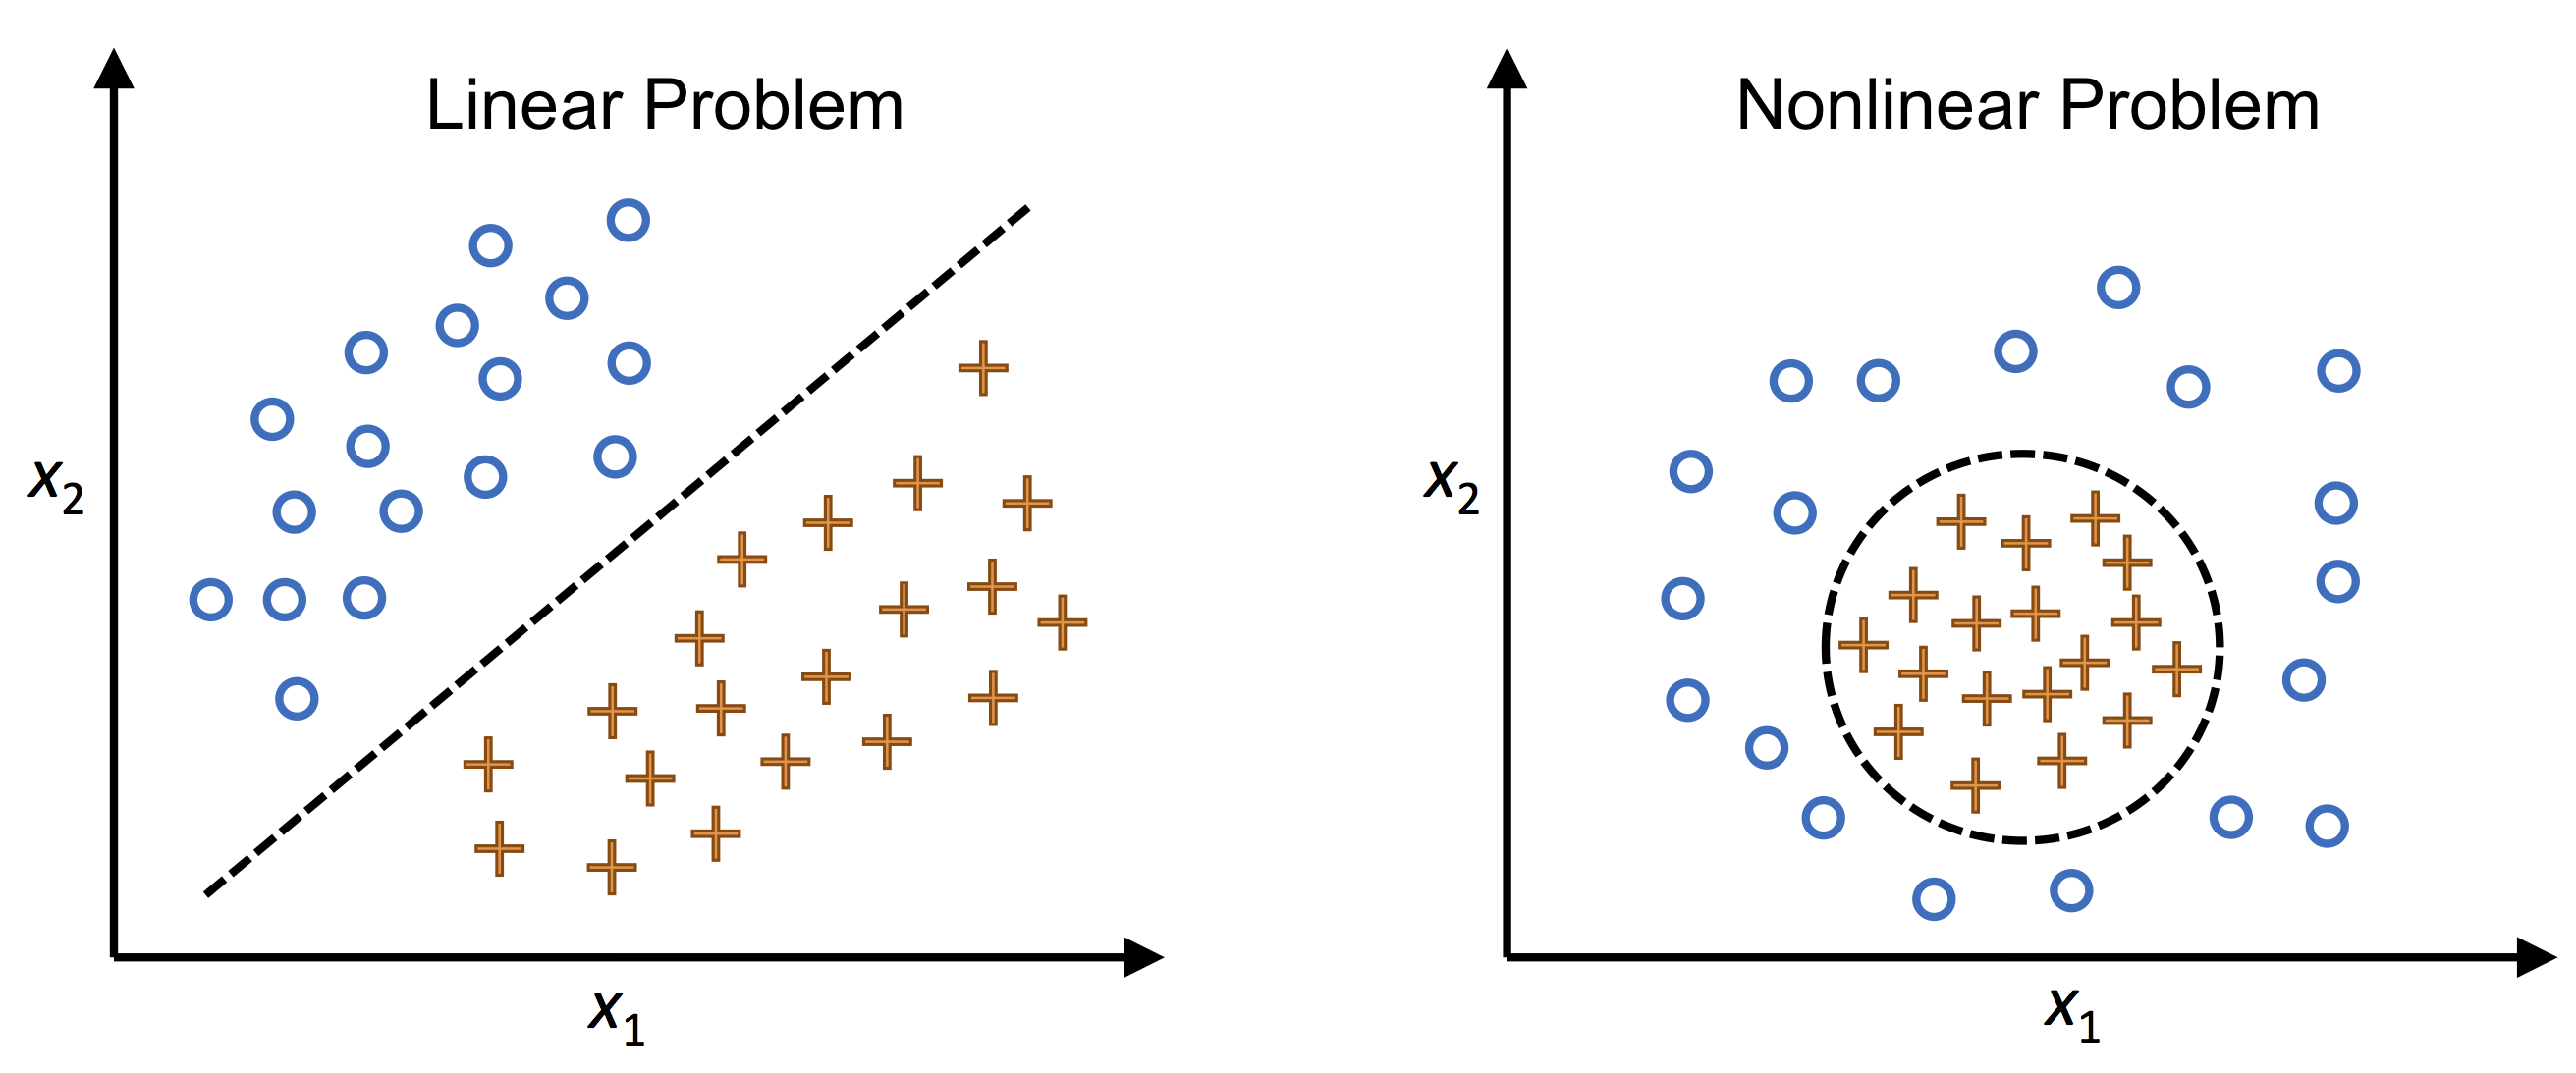
\includegraphics[width=100mm]{img/day05/fig03.png}
        \end{center}
    \end{figure}
\end{frame}

\begin{frame}{カーネル主成分分析}
    カーネルSVMと同様に非線形問題を得には、より高次元の新しい特徴量へ射影し、
    そこで線形分離可能な状態にする。データ点をより高い\(k\)次元に写像するために、
    非線形の射影関数\(\phi\)を定義した。
    \begin{equation*}
        \phi : \mathbb{R}^d \rightarrow \mathbb{R}^k (k \gg d) 
    \end{equation*}
    例えば、\(d\)を次元の数、\(\bm{x}\)を\(d\)この特徴量からなる列ベクトルとし、
    二次元の特徴量のベクトルが\(\bm{x} \in \mathbb{R}^d\)があるとすれば、
    3次元空間に次のように写像する。
    \begin{equation*}
        \bm{x} = [x_1, x_2]^T
    \end{equation*}
    \begin{equation*}
        \downarrow \phi
    \end{equation*}
    \begin{equation*}
        \bm{x} = [x_{1}^{2},\sqrt{2 x_1 x_2} ,x_{2}^{2}]^T
    \end{equation*}
    これで、標準のPACで低次元に変換することで線形分離を行うことができる。
\end{frame}

\begin{frame}{カーネルトリック}
    しかし、この方法では計算コストが非常に高いため、カーネルトリックを使用して、
    高次元へ写像することなく、元の特徴量において、2つの高次元の特徴量の類似度を計算できる。
    標準のPCAでは2つの特徴量\(j,k\)の間の共分散を次のように計算した。
    \begin{equation*}
        \sigma_{jk} = \frac{1}{n} \sum_{i=1}^{n} (x_{j}^{(i)} - \mu_j) (x_{k}^{(i)} - \mu_k)
    \end{equation*}
    特徴量を標準化すると、\(\sigma_j, \sigma_k\)の場合に平均値0が中心となる。
    このため、式を次のように簡略化できる。
    \begin{equation*}
        \sigma_{jk} = \frac{1}{n} \sum_{i=1}^{n} x_{j}^{(i)} x_{k}^{(i)}
    \end{equation*}
    よって共分散行列\(\bm{\sigma}\)は次のように計算できる。
    \begin{equation*}
        \bm{\sigma} = \frac{1}{n} \sum_{i=1}^{n} \bm{x}^{(i)} \bm{x}^{(i)T}
    \end{equation*}
\end{frame}

\begin{frame}{カーネルトリック}
    元の特徴量空間でのデータ点間の内積を、\(\phi\)を使って非線形の特徴量への組み合わせに変換できる。
    \begin{equation*}
        \bm{\sigma} = \frac{1}{n} \sum_{i=1}^{n} \phi(\bm{x}^{(i)}) \phi(\bm{x}^{(i)})^T
    \end{equation*}
    そして、次の方程式を解くことで固有値\(\lambda\)と固有ベクトル\(\bm{\nu}\)を取り出すことができる。\\
    \begin{equation*}
        \bm{\sigma} \bm{\nu}  = \lambda \bm{\nu} 
    \end{equation*}
    \begin{equation*}
        \Rightarrow \frac{1}{n} \sum_{i=1}^{n} \phi(\bm{x}^{(i)}) \phi(\bm{x}^{(i)})^T \bm{\nu}  = \lambda \bm{\nu} 
    \end{equation*}
    \begin{equation*}
        \Rightarrow \bm{\nu} = \frac{1}{n \lambda} \sum_{i=1}^{n} \phi(\bm{x}^{(i)}) \phi(\bm{x}^{(i)})^T \bm{\nu}
        = \frac{1}{n} \sum_{i=1}^{n} \bm{a}^{(i)} \phi(\bm{x}^{(i)})
    \end{equation*}
    \(\bm{a}\)を取得するには、カーネル(類似度)行列\(\bm{K}\)の固有ベクトルを抽出すればよい。
\end{frame}

\begin{frame}{カーネル行列}
    まず、共分散行列を行列表記法で記述する。この場合、\(\phi(\bm{X}) \in \mathbb{R}^{n \times k} \)
    \begin{equation*}
        \bm{\sigma} = \frac{1}{n} \sum_{i=1}^{n} \phi(\bm{x}^{(i)}) \phi(\bm{x}^{(i)})^T = 
        \frac{1}{n} \phi(\bm{X})^T \phi(\bm{X})
    \end{equation*}
    これにより、固有ベクトル方程式を次のように記述できる。
    \begin{equation*}
        \bm{\nu} = \frac{1}{n} \sum_{i=1}^{n} \bm{a}^{(i)} \phi(\bm{x}^{(i)})
        = \frac{1}{n} \phi(\bm{X})^T \bm{a} 
    \end{equation*}
    \(\bm{\sigma} \bm{\nu}  = \lambda \bm{\nu} \)であるため、次のようになる。
    \begin{equation*}
        \frac{1}{n} \phi(\bm{X})^T \phi(\bm{X}) \phi(\bm{X})^T \bm{a}  = \lambda \phi(\bm{X})^T \bm{a} 
    \end{equation*}
\end{frame}

\begin{frame}{カーネル行列}
    両辺に左から\(\phi(\bm{X})\)をかけると、次の結果を得ることができる。
    \begin{equation*}
        \frac{1}{n} \phi(\bm{X}) \phi(\bm{X})^T \phi(\bm{X}) \phi(\bm{X})^T \bm{a}  = \lambda \phi(\bm{X}) \phi(\bm{X})^T \bm{a} 
    \end{equation*}
    \begin{equation*}
        \Rightarrow \frac{1}{n} \phi(\bm{X}) \phi(\bm{X})^T \bm{a}  = \lambda \bm{a} 
    \end{equation*}
    \begin{equation*}
        \Rightarrow \frac{1}{n} \bm{K} \bm{a}  = \lambda \bm{a} 
    \end{equation*}
    \(\bm{K}\)は類似度(カーネル)行列であり、左辺の行列式\(\phi(\bm{X}) \phi(\bm{X})^T\)を置換できる。
    \begin{equation*}
        \bm{K} = \phi(\bm{X}) \phi(\bm{X})^T
    \end{equation*}
\end{frame}

\begin{frame}{カーネル行列}
    非線形SVMのように、カーネルトリックを使うことによって、
    データ点\(x\)の関数\(\phi\)同士の内積の計算をカーネル関数\(\mathcal{K}\)によって回避する。
    よって、明示的な固有ベクトルの計算は不要。\\
    \vspace{1em}
    \begin{equation*}
        \mathcal{K}(\bm{x}^{(i)}, \bm{x}^{(j)}) = \phi(\bm{x}) \phi(\bm{x})^T
    \end{equation*}
    \vspace{1em}\\
    カーネルPCAの後に取得するのは、それぞれの成分にすでに射影されたデータ点である。
    標準的なPCAとは異なり、変換行列を生成しない。
\end{frame}

\begin{frame}{カーネル行列}
    よく使われるカーネルは次のとおりである。
    \begin{itemize}
        \item 多項式カーネル。\(\theta\)は閾値、\(P\)はユーザが指定しなければならない指数。
        \begin{equation*}
            \mathcal{K}(\bm{x}^{(i)}, \bm{x}^{(j)}) = (\bm{x}^{(i)T} \bm{x}^{j}+\theta)^P
        \end{equation*}
        \item 双曲線正接カーネル。
        \vspace{1em}
        \begin{equation*}
            \mathcal{K}(\bm{x}^{(i)}, \bm{x}^{(j)}) = \tanh(\eta \bm{x}^{(i)T} \bm{x}^{j}+\theta)
        \end{equation*}
        \item 動径基底関数(RBF)またはガウスカーネル。次の頁で説明。
        \begin{equation*}
            \mathcal{K}(\bm{x}^{(i)}, \bm{x}^{(j)}) = 
            \exp (- \frac{\Vert\bm{x}^{(i)} - \bm{x}^{(j)}\Vert^2}{2 \sigma^2 })
        \end{equation*}
    \end{itemize}
\end{frame}

\begin{frame}{カーネル行列}
    これまでの内容をまとめる。RBFカーネルPCAの実装は次の3つにまとめることができる。
    \begin{enumerate}
        \item カーネル(類似度)行列\(\bm{K}\)を計算し、次の計算を行う。
        \begin{equation*}
            \mathcal{K}(\bm{x}^{(i)}, \bm{x}^{(j)}) = 
            \exp (- \frac{\Vert\bm{x}^{(i)} - \bm{x}^{(j)}\Vert^2}{2 \sigma^2 })
        \end{equation*}
        この計算をデータ点のペアごとに行う。
        \begin{equation*}
            \bm{K} = 
            \begin{bmatrix}
                \mathcal{K}(\bm{x}^{(1)}, \bm{x}^{(1)}) & \mathcal{K}(\bm{x}^{(1)}, \bm{x}^{(2)}) & \cdots  & \mathcal{K}(\bm{x}^{(1)}, \bm{x}^{(n)}) \\
                \mathcal{K}(\bm{x}^{(2)}, \bm{x}^{(j)}) & \mathcal{K}(\bm{x}^{(1)}, \bm{x}^{(2)}) & \cdots  & \mathcal{K}(\bm{x}^{(2)}, \bm{x}^{(n)}) \\
                \vdots  & \vdots  & \ddots   & \vdots  \\
                \mathcal{K}(\bm{x}^{(n)}, \bm{x}^{(1)}) & \mathcal{K}(\bm{x}^{(n)}, \bm{x}^{(1)}) & \cdots  & \mathcal{K}(\bm{x}^{(n)}, \bm{x}^{(n)}) \\
            \end{bmatrix}
        \end{equation*}
        たとえば、訓練データが100個存在する場合、カーネル行列は100\(\times\)100次元。
    \end{enumerate}
\end{frame}

\begin{frame}{カーネル行列}
    \begin{enumerate}
        \item 元の特徴量は標準化により平均が0であるが、射影後の特徴量は平均が
        0であることが保証できないので、以下の式を使ってカーネル行列の\(K\)の中心化を行う。
        \begin{equation*}
            \bm{K}^{'} = \bm{K} - 1_n \bm{K} - \bm{K} 1_n \bm{K} 1_n
        \end{equation*}
        \(1_n\)はすべての値が\(\frac{1}{n}\)に等しい\(n \times n\)の行列である。
        \vspace{1em}
        \item 対応する固有値に基づき、\(k\)個のベクトルを収集する。
        標準のPCAとは反対に、固有ベクトルは主成分軸ではなく、
        それらの軸に射影されているデータ点である。
    \end{enumerate}

\end{frame}

\end{document}